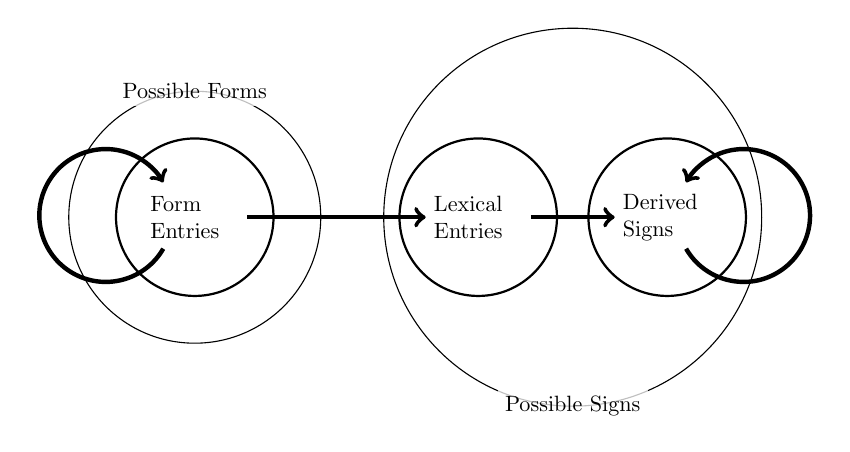
\begin{tikzpicture}[scale=0.8, every node/.style={transform shape}]
  \draw (0,0) circle (3) (0,-3) node [fill=white,fill opacity=0.75,text opacity=1] {Possible Signs};
  \draw[thick] (1.5,0) circle (1.25) (1.5,0) node (a) [fill=white,fill opacity=0.75,text opacity=1,text width=4em] {Derived Signs};
  \draw[thick] (-1.5,0) circle (1.25) (-1.5,0) node (b) [fill=white,fill opacity=0.75,text opacity=1,text width=4em] {Lexical Entries};
  \draw (-6,0) circle (2) (-6,2) node [fill=white,fill opacity=0.75,text opacity=1] {Possible Forms};
  \draw[thick] (-6,0) circle (1.25) (-6,0) node (c) [fill=white,fill opacity=0.75,text opacity=1,text width=4em] {Form Entries};

  \draw[->,ultra thick] (c) to (b);
  \draw[->,ultra thick] (b) to (a);
  \draw[->,ultra thick] (-6.5,-0.5) arc (330:30:30pt);
  \draw[->,ultra thick] (1.8,-0.5) arc (-150:150:30pt);

\end{tikzpicture}

%%% Local Variables:
%%% mode: latex
%%% TeX-master: "../../morphology"
%%% End:
